This chapter goes in detail about the architecture of the logical
planing of a query. Query planning is based on an A*-like search
algorithm for through the space of partial plans. We initially
describe the fundamental computational structures that facilitate this
search and their unique properties that allow us the necessary
flexibility. Then we discuss the basic backtracking algorithm and the
way the graph is traversed. We move on to discussing the garbage
collection that generates plan fragments that allow the plan to free
up space in the underlying storage. Finally we talk about the cost
model that guides the evolution of the plan.
\section{HCntT logic monad}

The FluiDB planner is designed in terms of a backtracking search
algorithm that searches in the space of subplans for an optimal (or
good-enough) plan. Because the algorithm involves a lot of complicated
heuristics it is important that a powerful underlying model is
deployed that matches the purely functional infrastructure in which
FluiDB is written.  We require a monad that supports both weighted
search and soft cuts. Because none of the solutions we dound in the
literature support both we we developed the \hask{HCntT} backtracking monad
that is described in this section.

\subsection{Background}

Monads for backtracking in a functional context have been proposed in
various incarnateions.  The most common monad that encapsulates
\hask{ListT m a = forall b . (a -> m b -> m b) -> m b -> m b}, also
dubbed the Church encoding of lists or an application of the Cayley
theorem on list, first proposed (in an untyped format in scheme) by
\cite{haynesLogicContinuations1987}, but most authors cite
\cite{hinzeDerivingBacktrackingMonad2000a} which seems to have
redescovered an application of the concpetsin 2000, and also
\cite{kiselyovBacktrackingInterleavingTerminating} who focused on a
notion of fairness in backtracking. As shown in
\cite{kidneyAlgebrasWeightedSearch2021} this representation has
\(O(n^2)\) BFS complexity.

The other common representation of a list transformer, is the more
straightforward

\begin{haskellcode}
newtype ListT m a = ListT (Maybe (a,ListT m a))
\end{haskellcode}

Which mirrors precisely the idea behid MonadLogic from
\cite{kiselyovBacktrackingInterleavingTerminating}. As demonstrated in
listing \ref{lst:monad_logic} the MonadLogic able to cons(\hask{reflect})
and uncons(\hask{msplut}).

\begin{code}
\begin{haskellcode}
class MonadPlus m => MonadLogic m where
  msplit :: m a -> m (Maybe (a,m a))
  -- ... other methods are defined in terms of msplit

reflect :: Maybe (a,m a) -> m a
reflect Nothing = mzero
reflect Just (a,as) = pure a <|> as

-- msplit >=> reflect == return
\end{haskellcode}
  \caption{\label{lst:monad_logic}The logic monad typeclass}
\end{code}

In \cite{kiselyovBacktrackingInterleavingTerminating}, on top of this
framework they build an interleave and a monadic bind operator that
works with it to make computation be slightly more "fair".
Interleaving is fair between two computations, when more than two are
involved, half the time goes to the first computation, out of the half
that is left, half (\(1/4\) of the total) goes to the second, out of the
\(1/4\) left, half (\(1/8\)) goes to the third and so on. While this
powerseries that describes the way the way resources are allocated to
branches may seem arbitrary, in practice it may mean the difference
between terminating and non-terminating computations. For example the
code in listing \ref{lst:list_logic_example} can be translated to something like the
code in listing \ref{lst:interl_logic_example} which does terminates due to the fact that
while it does not give the same change to all the branches it does not
completely starve any of them.

\begin{code}
\begin{haskellcode}
nonTerm :: [(Int,Int,Int)]
nonTerm = do
  (a,b,c) <- (,,) <$> genNaturals <*> genNaturals <*> genNaturals
  guard $ a + b - c == 10
  return (a,b,c)
\end{haskellcode}
  \caption{\label{lst:list_logic_example}Using a simple list to drive
    non-determinism is implicitly equivalent to a DFS algorithm which
    in many useful cases does not terminate.}
\end{code}

\begin{code}
\begin{haskellcode}
interleaveTest :: [(Int,Int,Int)]
interleaveTest = runLogic @[] $ do
  (a,b,c) <- genNaturals >*< genNaturals >*< genNaturals
  guard $ a + b - c == 10
  return (a,b,c)
\end{haskellcode}
  \caption{\label{lst:interl_logic_example}Interleaving (in this
    example \hask{>*<}) is not \emph{actually} fair in the sense that
    it does not give all the processes}
\end{code}

So can we do better than terminating? Sometimes we can with weighted
search. Weighted search refers to the backtracking search where we
apply weights, or priority, to the branches. Branches with higher
priority are scheduled before branches with lower priority. A sketch
of the API is demonstrated in listing \ref{lst:halt_example}. The
backtracking monad implements the \hask{halt} operation (called
\hask{tell} in \cite{kidneyAlgebrasWeightedSearch2021}, presumably to
echo the \hask{MonadWriter} interface) which accepts a value
indicating the priority of the current branch and yields control to
the scheduler. The scheduler then passes control to the highest
priority branch. The value passed to \hask{halt} must implement a
monoid such that the priority of a branch is the concatenation of all
values passed to halt up to that point.

\begin{code}
\begin{haskellcode}
  -- | Non-deterministically return an integer but before that pass
  -- control to the scheduler which prioritizes branches based on a
  -- total sum which it tries to minimize.
  stream :: (HeapKey h ~ Sum Int,IsHeap h,Monad m) => HCntT h r m Int
  stream = go 0 where
    go i = do
      halt $ Sum i
      return i <|> go (i+1)

  -- | Non-deterministically choose three numbers and only keep the
  -- branches that satisfy a + b - c == 10. Avoid diverging by prefering
  -- branches for which the sum of the numbers is minimum.
  test2 :: IO [(Int,Int,Int)]
  test2 = takeListT 5 $ dissolve @(CHeap (NonNeg Int)) $ once $ do
    (a,b,c) <- (,,) <$> stream <*> stream <*> stream
    guard $ a + b - c == 10
    return (a,b,c,x)
  -- > test
  -- [(5,5,0),(6,4,0),(5,6,1),(6,5,1),(6,6,2)]
\end{haskellcode}
  \caption{\label{lst:halt_example}Prioritise branches that we want to
    be executed first.}
\end{code}

With that in mind, for the FluiDB planner we require that our logic
framework supports the following features:

\textbf{Weighted search:} Not all plans that match our criteria, i.e. that
solve the query within the space are equally admissible. We need to
find as good plans as possible and we do not want the planner to spend
time looking into plans that are unlikely to be efficient. For that
reason neither breadth-first nor depth-first traversals are ideal for
our purpose. We need a robust way to search in a weighted manner.

\textbf{Soft-cut/either:} As we will see in more detail in the next section,
the planner is initially optimistic about being able to materialize a
node until it hits the budget limit. If the budget turns out to be
large enough FluiDB should completely disregard the the branch with
the node should be completely forgotten about. The reason is that the
later a GC happens the more options it will have and therefore the
better job it will do. To achieve that we implement an operator we dub
\hask{<//>} (pronounced \emph{eitherl}) which is similar to prolog's soft-cut.

\textbf{Once:} In the context of non-weighted search it is fairly
straightforward to demand that a subcomputation yields no more than
one value (prolog's \hask{once}). Simply run the entire computation
in-place requesting one result and if it doesn't fail return that
result. This approach can still work with weighted but we would like
the \hask{halt} calls inside the computation to have global effect for the
scheduler. In other words we want the scheduler to be able to
interleave this branch with other branches while preserving the
semantics of \textbf{once}.

None of the work we could find easily implements all the above
features simuntaneous for the FluiDB planner so we implement yet
another backtracking monad transformer, \hask{HCntT}.


\subsection{The HCntT monad}

The \hask{HCntT} monad combines the powers of delimited continuations and
much like \cite{kidneyAlgebrasWeightedSearch2021} it rsearches the
result in layers (see listing \ref{lst:hcntt_def}).

\begin{code}
\begin{haskellcode}
type HCntT h r m = ContT (HRes h m r)
  (ReaderT (HeapKey v)
   (StateT (CompState h r m) m))

newtype HRes h m r = HRes (Tup2 (h (Brnch h r m)),[r])
type Brnch h r m = ReaderT (HeapKey v)
  (StateT (CompState h r m) m) (HRes h m r)
\end{haskellcode}
\label{lst:hcntt_def}
\caption{The \hask{HCntT} monad transformer allows continuation based
  non-determinism that allows switching between branches.}
\end{code}

Here we use the continuation monad to capture the rest of the
compuation and be able to access the final result from the scope of
each operator. The result is represented as \hask{HRes} which is an
intermediate layer of the continuation. Returning empty results should
be passing. It contains a heap of halted branches and a list of
concrete evaluated valies. The heap type is parametric to allow
flexibility with respect to how to best handle the particular key
types (see listing \ref{lst:heap_def}). The heap is required to be stable,
i.e. items with the same key are returned in the order they were
inserted. The HeapKey \hask{mempty} must be less than (higher priority) all
other \hask{HeapKey} s.

\begin{code}
\begin{haskellcode}
class (forall v . Monoid (h v),Functor h,Monoid (HeapKey h),Ord (HeapKey h))
  => IsHeap h where
  type HeapKey h :: *

  popHeap :: h v -> Maybe ((HeapKey h,v),h v)
  singletonHeap :: HeapKey h -> v -> h v
  maxKeyHeap :: h v -> Maybe (HeapKey h)
\end{haskellcode}
\label{lst:heap_def}
  \caption{We parameterize over heaps to allow the
    user to decide an efficient priority queue for the branches.}
\end{code}

A halted computation branch, denoted as \hask{Brnch} is simply a
computation that evalautes to HRes. The computation must be able to
interact with CompState as required by the infrastructure supporting
\hask{<//>}.

The \hask{HCntT} on its own is not a very useful object, it needs to
be \emph{dissolved} so the values can be used. Disolution (listing
\ref{lst:dissolve_func}) is the process of turning an HCntT value to a
\hask{ListT} value. The \hask{ListT} will lazily produce just as many
results as are required, and of course just as many effects as
required, and not more. This indicates that the process of building
comptuatins is composable but not incremental. The price of the
\hask{<//>} combinator that we described is that, unlike in other
non-continuation based monad, once we start drawing results from the
computation we can not apply further constraints on the resulting
objects. Contrast that with the case of \hask{ListT} where we can draw
the first couple of results and then use the rest in a different
computation.

\begin{code}
\begin{haskellcode}
dissolve :: (IsHeap h,Monad m) => HCntT h r m r -> ListT m r
\end{haskellcode}
  \caption{\label{lst:dissolve_func}Disolution is the process of
    turning an \hask{HCntT} computation into a \hask{ListT}.}
\end{code}

The way disolution works then (listing \ref{lst:dissovle_algo}) is to first
commit to the computation constructed by applying the continuation and
obtaining an \hask{HRes}. If \hask{HRes} provides concrete results they are
yielded one by one into \hask{ListT}. Then, if the heap is not empty, the
highest priority branch is popped and scheduled to run until it yields
a new \hask{HRes}. The concrete results are yielded into \hask{ListT} and the
new heap is combined with the old one. Scheduling a branch entails
running the reader layer of the monad transformer using its pervious
value. As we will see, halting the branch will update that value
incrementally.

We use \hask{Tup2} (a functor that is simply \hask{data Tup2 = Tup2 a
  a}) in the type of \hask{HRes} to allow us to be flexible on whether
we use BFS or DFS search among the same-priority branches. As
mentioned when describing the heap, a valid heap for \hask{HCntT} must
be stable. While this is a weighted search, it remains a question of
how the options that have the same priority should be ordered. If we
had just one heap, appending the newly produced heaps to the left
would make for a depth first traversal of the same-priority search
space while appending on the right would result in a breath first
traversal. We want the operators to have the flexibility to decide on
which side each branch should be appended and for that reson the
\hask{HRes} actually contains two heaps: one appended to the left
(DFS), and one to the right (BFS). This is of particular importance to
the correct implementtion of \hask{<//>} as we will see shortly.

\begin{code}
\begin{pycode}
def dissolve(branches):
    while len(branches) > 0:
        priority,best_branch = branches.pop()
        (sub_branches_left,sub_branches_right),results = best_branch.run()
        branches = sub_branches_left + brances + sub_branches_right
        for r in results:
            yield r
\end{pycode}
  \caption{\label{lst:dissovle_algo}The dissolution algorithm in
    pseudo-python}
\end{code}


In the following we will briefly describe the implementations of
various combinators of \hask{HCntT}.

\subsubsection{Alternative/MonadPlus}

The most fundamental combinator for any backtracking monad is the one
splitting branches, the implementation of \hask{Alternative} or,
equvalently in our case, \hask{MonadPlus}. The implementation for \hask{HCntT}
is fairly straightforward (listing \ref{lst:alternative_impl} ) is fairly
straightforward: for \hask{empty} or \hask{mzero}, which indicates failure of a
branch, simply disregards the continuation and returns an empty
\hask{HRes}. The \hask{mplus} or \hask{<|>} simply returns an \hask{HRes} with only the
two alternative branches having maximum priority (i.e. \hask{mempty ::
HeapKey h}) and bounded to the current continumation. Both those
branches are pushed from the right so that they are scheduled before
other same-priority branches.

\begin{code}
\begin{haskellcode}
instance (IsHeap h,Monad m) => Alternative (HCntT h r m) where
  ContT m <|> ContT m' = ContT $ \f -> return
    $ HRes (Tup2 (h (m f) <> h (m' f)) mempty,[])
    where
      h = singletonHeap mempty
  empty = ContT $ const $ return emptyHRes
\end{haskellcode}
  \caption{\label{lst:alternative_impl}The implementation for
    \hask{Alternative} is the same as the implementation for
    \hask{MonadPlus}.}
\end{code}


\subsubsection{halt: passing control to the scheduler}

We mentioned the \hask{halt} \hask{HCntT} process. Because we want to
be able to transform the \hask{HCntT} monad we define the class of
\hask{MonadHalt} that can support this operation. Most common monad
transformers of \hask{HCntT} can trivially support halt. The
implementation of \hask{halt} for \hask{HCntT} itself is demonstrated
in listing \ref{lst:halt_class}. The provided priority is offset by the
previous priority of the branch.

\begin{code}
\begin{haskellcode}
class Monad m => MonadHalt  m where
  type HaltKey m :: *
  halt :: HaltKey m -> m ()

instance (Monad m,IsHeap h) => MonadHalt (HCntT h r m) where
  type HaltKey (HCntT h r m) = HeapKey h
  halt v = ContT $ \nxt -> do
    v' <- asks (v <>)
    return $ HRes (Tup2 (singletonHeap v $ nxt ()) mempty,[])
\end{haskellcode}
  \caption{\label{lst:halt_class}The halt process yields updates the
    priority of the branch and yields execution to the scheduler.}
\end{code}


\subsubsection{Soft-cut/eitherl}

The \hask{<//>} (pronounced eitherl), \hask{left <//> right} runs the
left hand side operand (primary) and if no values are produced in the
\emph{entire} computation based on that, only then does it try to
evaluate the right hand side (fallback). \hask{HCntT} does not
guarante that the right hand side will be scheduled immediately after
it realizes that there are no solutions, but it does guarantee that it
will be scheduled before it moves on to a new priority. In other words
it is only guarantted that the priority of the fallback branch will
tie the last failing branch of the left hand side in terms of
priority, but if there are other branches that tie, there is no
guarantee of how those will be scheduled.

There are two challenges that our particular feature set imposes to
implementing this:

\begin{itemize}
\item We want \hask{<//>} to operate on the entire operation, unlike
  \cite{kiselyovBacktrackingInterleavingTerminating} that makes the
  decision o whether to run the fallback solely based on whther the
  left hand side returns a value.
\item In the context of a weightedx search control needs to be able to
  escape a branch that passes through the left hand side operand
  before it is exhausted. Therefore we can not simply dissolve the
  left hand side and reconstruct it. But then how would the operator
  know when the branches are exhausted?
\end{itemize}

We solve these problems with the use of a special kind of branch we
call a \emph{marker}, and a global state. Since branches are arbitrary
processes we equip them with access to global state (local to the
computation), a lookup table (\hask{CompState}) full of fallback
branches. The main ideas is that a fallback branch corresponds to an
entry int the lookup table. This entry is modified accordingly by the
children of the right hand side. At the time of the cut we push a
marker into the heap with priority lower than the child branches so
that when it is scheduled it will perform some checks based on the
lookup table entry and schedule the fallback function if all the
children branches have finished whithout a result.

We will see in a bit how the contents of the lookup table are updated
and how new, lower priority markers are pushed in the heap. For now
consider that each marker may be superseded by a lower priority marker
rendering it a invalid. At any time there is exactly one valid marker
per active fallback and it is denoted as such by the fallback entry in
the lookup table. The rest of makers are invalid and should be
equivalent to noops.

More precisely about the internals of the marker processes, each one
refers to a location in the lookup table via its closure. Also each
marker is uniquely identifiable so each valid entry in the lookup
table references one marker. Specifically the lowest priority one that
corresponds to it. When the marker is scheduled it looks up the
fallback branch entry in the table and checks if the entry also refers
to that marker. There are 3 possible scenaria that may play out at
this point:

\begin{itemize}
\item The fallback entry in the table has been invalidated by a branch
  that yielded a result. In this case the marker is invalid and just
  returns.
\item The fallback entry is valid but does not correspond to the
  scheduled marker. This means due to the left hand side branch
  spawning low priority sub-branches, another marker has been inserted
  to (possibly) trigger the fallback at some time in the future. The
  current marker is invalid
\item The fallback location is valid and corresponds to the scheduled
  marker. This means that it is time fallback process needs to be run
  and removed from the table.
\end{itemize}

But what is the lifecycle of the fallback entries? When an exprssion
\hask{A <//> B} appears we create a new fallback entry in the lookup
table containing \hask{B} and recursively "infect" all spawned
sub-branches of \hask{A} to perform the following actions immediately
after they generate new branches and results:

\begin{itemize}
\item If there is at least one valid result invalidate the fallback in
  the lookup table and stop infecting child branches with the
  currently described hook.
\item If the fallback is invalid it means there have already been
  valid results that rendered the fallback obsolete. Stop infecting
  sub-branches.
\item If none of above happened check the priority of the last marker
  corresponding to the fallback (registerd in the lookup table
  entry). If it is strictly lower than the lowest priority subbranch
  do nothing because there is a well placed marker to handle
  it. Otherwise create a new marker of the same priority as the lowest
  priority subbranch and put it in the right-append heap. This way we
  know it will be scheduled AFTER the last branch relating to the
  fallback.
\end{itemize}


It is demonstrated in figure \ref{fig:marker_branches}

\begin{figure}[p]
  \begin{tikzdiagram}
    \tikzset{b/.style={circle,draw,minimum size=1cm}};
    \tikzset{m/.style={circle,draw,minimum size=1cm, fill=gray!10}};
    \tikzset{node/.style={rectangle}};
    \tikzstyle{background}=[rectangle, fill=gray!10, inner sep=0.2cm]

    \node[node] (sep) {};

    \newcommand{\s}{\node[node] {};}
    \matrix (tbl) [above of = sep,background, nodes={align=center,minimum height=2em}]{
      \s \& \node {...}; \& \s \\
      \node[node] (rec_data){\(b_{fallback}\)}; \&
      \node[node] (rec_id) {\(id\)}; \&
      \node[node] (rec_br) {\(m_3\)}; \\
      \s \& \node {...}; \& \s \\
    };
    \node[node] (tbl_label) [left=of tbl] {Fallback branch table:};

    \node[node] () [fit=(rec_data) (rec_br),draw] {};

    \matrix [column sep = 0.3cm, below = 1cm of sep] {

      \node[node] (heap_lbl) {Branch heap:}; \&
      \node[b] (b1)  {\(b_{1}\)}; \&
      \node[b] (b2)  {\(b_{2}\)}; \&
      \node[m] (m1)  {\(m_{1}\)}; \&
      \node[b] (b4)  {\(b_{4}\)}; \&
      \node[m] (m2)  {\(m_{2}\)}; \&
      \node[b] (b6)  {\(b_{6}\)}; \&
      \node[m] (m3)  {\(m_{3}\)}; \&
      \node[b] (b8)  {\(b_{8}\)}; \&nppppnnn
      \node[b] (b9)  {\(b_{9}\)}; \\
    };
    \draw [dotted,-stealth] (m1) to (rec_id);
    \draw [dotted,-stealth] (m2) to (rec_id);
    \draw [-stealth] (m3) to [bend left =10] (rec_id);
    \draw  [-stealth] (rec_br)  to [bend left = 10] (m3);
  \end{tikzdiagram}
\caption{\label{fig:marker_branches}Marker "branches" are injected in
  the heap of prioritized branches to possibly trigger the fallback
  branch. Each marker gives the scheduler the opportunity to run a
  particular fallback branch. The entry of the fallback branch entry
  references the last marker so that only that one actually trigger
  the fallback branch. A child branch that succeeds removres the
  fallback entry so the final marker also fails to tigger the
  fallback.}
\end{figure}

There are some optimizations that can be implemented to avoid too many
lookups in the fallback table in the case of deep eitherl nesting that
take advantage of the fact that new markers for outer fallbacks may
only be created when new markers for inner fallbacks are
created. However, for FluiDB we did not find \hask{CntT} to be too bad of a
performance bottleneck so we leave it for future work.


\subsubsection{Once}

The \hask{once} operator runs the argument computation and stops once it
returns the first result. FluiDB uses \hask{once} to run the garbage
collector without exploding the search space. Generally the different
combinations of nodes that can be deleted is huge. We prune that by
space by settling for the first result the solver can find.

The way \hask{Once} is built on top of a concept we call a
\emph{nested scheduler}. It takse a computation (the \emph{nested
  computation}) and needs to know what to do in case of a success and
in case of complete failure (no more branches to run). The nested
scheduler is a process that \emph{always} returns a single case
subbranch. This subbranch has the priority of the highest priority
subbranch of the nested computation and when scheduled it internally
schedules the next branch of the nested process. When the process
yields results or fails completely the corresponding hook is
run. \hask{once} implements these hooks as "return the result and
stop" and as "propagate the failure" respecively. Since the
implementation of \hask{once} is fairly small it is provided along
with the types in listing \ref{lst:once_def}.

\begin{code}
\begin{haskellcode}
nested
  :: forall h m r a .
  (Monad m,IsHeap h)
  => (Tup2 (h (Brnch h r m)) -> r -> [r] -> HRes h m r)
  -> HRes h m r
  -> HCntT h r m a
  -> HCntT h r m a
nested success fail c = ...

once :: forall h m r a . (Monad m,IsHeap h) => HCntT h r m a -> HCntT h r m a
once = nested (\_h r _rs -> HRes (Tup2 mempty mempty,[r])) emptyHRes
\end{haskellcode}
\caption{\label{lst:once_def}The nested scheduler runs a subprocess within a single branch. Once is built on top of that to make sure the process stops once a result is returned.}
\end{code}


It is worth noting that nested schedulers are also applicable of
implementing \hask{<//>}. In the marker-based implementation we are
performing \(N\) lookups on the fields table, \(N\) being the nesting
of \hask{<//>} operators. Implementing it using nested schedulers, on the
other hand, means we are doing \(N\) pop/push pairs, one for each
nested heap. For FluiDB we use a slighltly too general notion of a
heap so we opt for the former.
\section{The planner}
\label{sec:planner}

\subsection{Traversing the graph}

The planner is the subsystem of FluiDB that given the state of the
QDAG and a target node to be materialized produces a logical plan that
will materialize the query.  Our notion of a logical plan is slightly
more specific them what is commonly considered a logical plan,
i.e. the RA representation of the query. In our case it is a sequence
of \emph{transitions} that are to be transpiled to C++ by the code
generator. There are three kinds of transitionse:

\begin{itemize}
\item t-node trigger that assumes the input n-nodes are materialized and
produces a subset of the output nodes.
\item t-node reverse trigger that assumes that the output nodes are materialized
\item n-node deletion
\end{itemize}

The planner operates by backtracking using \hask{CntT} monad. Each branch
mainains some branch-internal effects that are reified as monad
transformers on top of the \hask{CntT} defining the \hask{PlanT} monad
transformer (listing \ref{lst:plant_def}).

\begin{code}
\begin{haskellcode}
type PlanT t n m =
  StateT
    (GCState t n)
    (ReaderT (GCConfig t n)
     (ExceptT (PlanningError t n)
      (HCntT PlanHeap () m)))
\end{haskellcode}
  \caption{\label{lst:plant_def}The monad that defines all the useful
    effects used by the planner. \hask{GCConf t n} is an immutable,
    from the persepctive of the planner, configuration that includes
    the QDAG, the node sizes, etc. \hask{GCState t n} is state that is
    mutated and private to each branch of the planner like the
    materialized status of the nodes, the set of transitions
    registered so far and various caches. The \hask{PlanningError t n}
    is a planner specific type of error. The entirety of the result of
    planning is accumumated in \hask{GCState} so the result of
    backtracking is just unit (\hask{()}).}
\end{code}

It is important to clarify the way we use the term "materialized node"
(\hask{Mat} as opposed to "not materialized" -- \hask{NoMat}) from the planner's
perspective. A mapping of node states is passed to the planner at the
beginning of the planning process. This mapping indicates which nodes
are initially materialized. Then as transitions get registered update
the mapping is updated to reflect the effect that the plan so far
would have on the materialized relation set in storage. Since the
planner operates via backtracking (using the \hask{CntT} monad described),
each branch maintains its own mapping of node states and therefore
considers a different set of materialized nodes.

We maintain the partial plan (sequence of transitions) as part of the
state of each of the planners branches. Registering a transition means
that a transition is added to the partial plan.

The main loop of the planer is a recursive process of asseerting that
nodes are materialized. If the node is already materialized the
assertion succeeds, if not the planner attempts to trigger, or reverse
trigger, a neighbouring t-node that would lead to the node being
materialized, asserting first that the input nodes of that transition
are materialized. In practice, due to intermediate n-nodes being
auxiliary and not corresponding to real nodes, we know that t-nodes
are organized in sequences that need to be triggered entirely or not
at all. For example (figure \ref{fig:example_metaop}) the intermediate
\(\lsemi\) nodes are not actually materialized as part of the join
operator. Equipped with this knowledge we organize the t-nodes into
\hask{MetaOps} (listing \ref{lst:metaop_def}) that can atomically be triggered or
reverse triggered. \hask{MetaOps} also abstract the distinction between
triggering and reverse triggering as they expose a set of input, a set
of output nodes and a process that registers the correct transitions
once the \hask{MetaOp} is triggered. The process of asserting asserting an
n-node being materialized then becaomes the process of
non-deterministically selecting a \hask{MetaOp} with the node in question
in the output set. Before actually splicing the \hask{MetaOp} compiutation
we assert that the input set is materialized.


\begin{figure}[p]
\centering
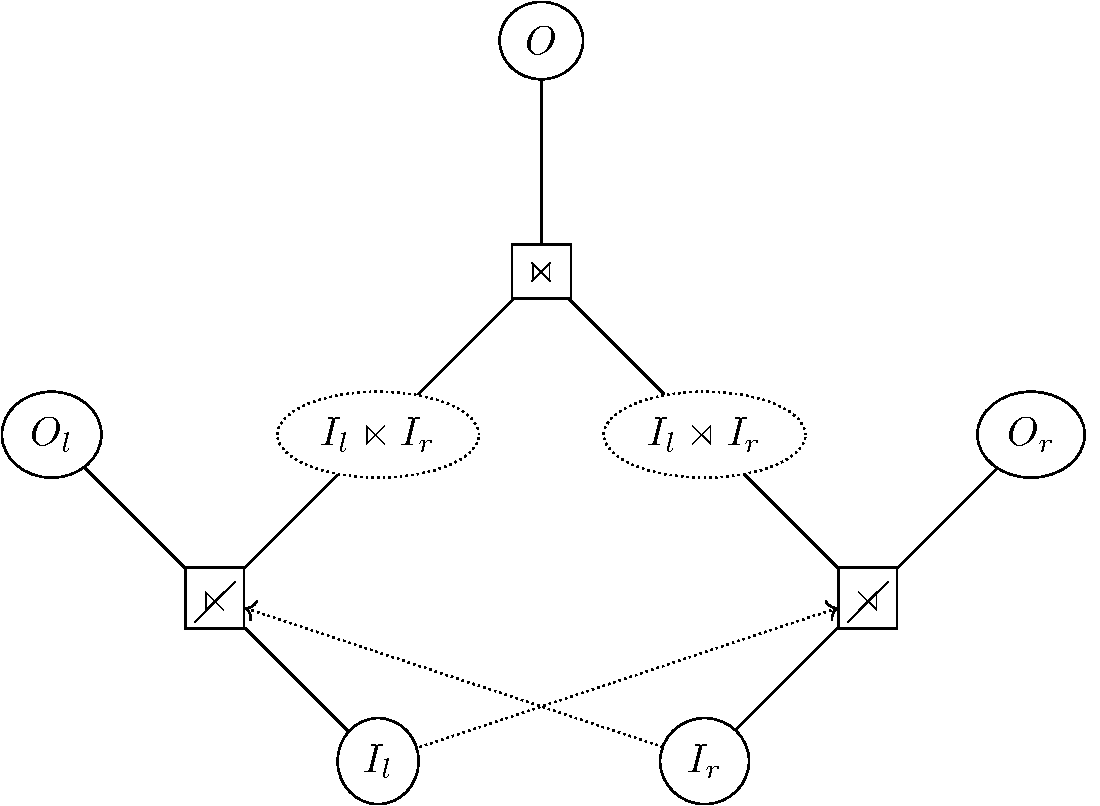
\includegraphics[width=.9\linewidth]{./imgs/example_metaop.pdf}
\caption{\label{fig:example_metaop}starting at node \(O\), the output
  of a join operation, we can derive three MetaOps that can
  materialize it.
  \(MetaOp\{in: \langle I_l, I_r \rangle, out: \langle O \rangle \}\),
  \(MetaOp\{in: \langle I_l, I_r \rangle, out: \langle O_l, O \rangle
  \}\),
  \(MetaOp\{in: \langle I_l, I_r \rangle, out: \langle O, O_r \rangle
  \}\),
  \(MetaOp\{in: \langle I_1, I_2 \rangle, out: \langle O_l, O, O_r
  \rangle \}\). Because trying all combinations of outputs explodes
  the seach space we always go for the largest and then let the
  garbage collector deal with the possible reprecussions. On the other
  hand to materialize \(I_l\) there is only one \hask{MetaOp} that
  relates to this cluster
  \(MetaOp\{in:\langle O, O_l \rangle, out: \langle I_l \rangle,
  interm: \langle I_l \lsemi I_r \rangle \}\)}
\end{figure}

\begin{code}
\begin{haskellcode}
data MetaOp t n = MetaOp {
  metaOpIn     :: NodeSet n,
  metaOpOut    :: NodeSet n,
  metaOpInterm :: NodeSet n,
  metaOpPlan   :: forall m' . Monad m' => PlanT t n m' [Transition t n]
  }
\end{haskellcode}
  \caption{\label{lst:metaop_def}A \hask{MetaOp} refers to input,
    output, and intermediate nodes that are involved in the set of
    operations it abstracts. Furthermore it contains a computation
    that registers and returns the transitions involved in the
    \hask{MetaOp}.}
\end{code}


Two questions should arise from the above description: a) how does the
planner avoid cycles where it recursively tries to materialize the
parents and then the children? and b) how does it know not to
materialize a node twice? Both those problems are addressed by
refining the possible states of the n-nodes (listing
\ref{lst:ismat_def}). Rather than being just \hask{Mat} or
\hask{NoMat}. We also disambiguate between \hask{Initial} and
\hask{Concrete} nodes. Nodes in the \hask{Initial} state are allowed
to change their materialization status. In contrast \hask{Concrete}
nodes have their state fixed with very few exceptions. Then, when a
node is asserted to be materialized its status is first checked and
followin scenaria are possible:

\begin{itemize}
\item the node's status found to be \hask{Concrete} and \hask{NoMat}
  and the branch immediately fails as it is not allowed to be set to
  materialized.
\item if it is \hask{Concrete} and \hask{Mat} the assertion simply
  succeeds
\item If it is \hask{Initial} and \hask{Mat} it is turned into
  \hask{Concrete} and \hask{Mat} and the assertion succeeds.
\item if the node's status is \hask{Initial} and also \hask{NoMat},
  two things need to happen: first the node is set \hask{Concrete} and
  \hask{NoMat} in order to avoid cycles, and the aforementioned
  process of finding a \hask{MetaOp} is carried out recusively in
  order to materialize the node.
\end{itemize}

\begin{code}
\begin{haskellcode}
data IsMat = Mat | NoMat
data NodeState =
  -- Concretified states are allowed to change only within the same
  -- lexical scope.
  Concrete IsMat
  -- Initial states are subject to change when encountered as a
  -- neighbour or by the GC.
  | Initial IsMat
\end{haskellcode}
  \caption{\label{lst:ismat_def}The different states that a node is
    allowed to be in.}
\end{code}


Once an n-node's is materialized and we start materializing its
siblings, it is important that the garbage collector (which we will be
discussing in the next section) does not delete said n-node.  To avoid
this problem, items materialized are set to \hask{Concrete Mat} until all
their siblings, that are inputs to the same \hask{MetaOp}, are
materialized. Once the \hask{MetaOp} is triggered and its output nodes are
set to the \hask{Concrete Mat} state the input nodes are set to \hask{Initial
Mat} as it is now safe for the garbage collector to remove them.

It is worth noting here the importance of every node in the depset
being completeley materialized before the process of materializing the
next one comences. The reason is that at any time a single trail of
parent nodes is marked as \hask{Concrete} and \hask{NoMat}, otherwise we can't
be sure whether a \hask{Concrete NoMat} node that renders a \hask{MetaOp}
non-triggerable is actually in the process of becoming materialized,
meaning that when that process succeeds the \hask{MataOp} under
consideration will be triggerable.

\subsection{Garbage collection}

One of the fundamental design decisions of FluiDB is that it is
commited to materializing all intermediate nodes and keeping them
around for as long as possible. In one hand the plan selected is
crafted so that the intermediate results are maximally useful for the
overall workload, on the other, when the available storage runs out,
the garbage collector mechanism selects the least useful nodes to be
deleted, creating free required for solving the query. In this section
we focus on the latter.

The garbage collector is triggered right before a \hask{MetaOp} is to be
triggered. It infers the space required for materializing the output
nodes and the space available to decide how much space is
required. Then it selects a subset of materialized nodes to delete in
order to make room for the new results. The selection process has two
hard constraints:

\begin{itemize}
\item The nodes being deleted must be \emph{deletable}, i.e. the
  node's state is \hask{Initial} and if the node is deleted it can be
  reconstructed from the remaining materialized nodes.
\item The nodes being deleted must not be required for the
  continuation of the current plan. We call these nodes
  \emph{protected}. For example, say we are planning for the query
  \(A \Join B\) and we have materialized \(A\) already but while
  materializing \(B\) the GC is triggered. \(A\) should not be in the
  repertoire of nodes the GC can delete under any circumstances.
\end{itemize}

Selecting a subset of nodes is not an easy problem so we follow a
simple heuristic and leave a proper solution for future work.

Large nodes are costly to create and therefore the larger the node,
the less inclined the planner is to create it, and the more useful it
is likely to be. With that in mind the heuristic we follow is for the
garbage collector to prioritise deleting small nodes over deleting
larger ones. The first order of business for the GC the is to find the
set of deletable nodes and sort them by size. It tries to delete them
one by one starting from the smaller ones and working its way up to
the larger ones. Every time a node is deleted it is possible that
other nodes that were previously established to be deletable lose that
property. For example if all nodes \(A\), \(\sigma_p A\), and
\(\sigma_{\neg p} A\) are \hask{Initial} and materialized, each one of
them can be materialized from the others and therefore all of them are
marked as deletable. If the GC deletes \(\sigma_p A\) first the other
two are no longer materializable as they depended on \(A\) to be
materializable.

Nodes that are established as non-deletable in this way are switched
from \hask{Initial} to \hask{Concrete} to avoid re-calculating their
materializability.

If after this process not enouch space was created, the GC resorts to
starting a new \emph{planner epoch}. When a new planner epoch begins all
the nodes states and transitions that were recorded since the last
planner epoch started are stashed into the epoch stack. The epoch
stack resides in the branch-local state (\hask{GCState}) and contains a map
of nodes to their states at the end of the epoch and a sequence of
transitions. When a new epoch is pushed into the stack a new mapping
of states is created according to the following rules:

\begin{itemize}
\item The materialization status does not change between epochs: All
  materialized nodes from the previous epoch are materialized in the
  new one materialized and all non-materialized nodes are still not
  materialized.
\item All non-protected \hask{Concrete} nodes become \hask{Initial}
  nodes.
\end{itemize}

The sequence of transitions for the new epoch is empty. The reason we
keep separate lists of transitions is, as we will see in more detail
in the code generation chapter, that the subset of output nodes that a
physical operation generates is established at the time of physical
planning based on the materialized nodes according to the epoch
corresponding to the transition.

An epoch contains all the important information about the state of the
planner. For this reason when an epoch is inserted in the stack it is
checked for equality against the other epochs in the stack. If two
equivalent epochs are inserted in the stack the branch fails
permanently as it means that there is a cycle.

This enables another optimization, the \emph{free-to-delete} nodes. As
mentioned previously the planner prioritizes the version of \hask{MetaOps}
that materializes all the outputs for example it will prioritize the
branch that followes \(MetaOp\{in=\langle A \rangle, out=\langle
\sigma_p A, \sigma_{\neg p} A \}\) over the on that follows
\(MetaOp\{in=\langle A \rangle, out=\langle \sigma_p A \}\). It is
rarely the case, however, that all the outputs are required. In the
example just mentioned then the former example, triggering the former
\hask{MetaOp} and then garbage collecting \(\sigma_{\neg p} A\) without it
being used is never desirable. For that reason we mark the node
\(\sigma_{\neg p} A\) as \emph{free-to-delete} as soon as it is created
based on the fact that it is not required. When the garbage collector
deletes free-to-delete nodes it does so without registering a deletion
transition. This way the physical planner will generate a plan where
\(\sigma_{\neg p} A\) is never created in the first place. All nodes
lose their free-to-delete status upon the creation of a new epoch.

The comprehensive algorithm for the GC is presented in listing
\ref{lst:gc_algo}

\begin{code}
\begin{haskellcode}
gc reqSize = do
  -- Try the current epoch and if that fails retry with a new epoch.
  return () <//> newEpoch
  -- find the deletable nodes and sort them by size
  deleteables <- sortOnM getNodeSize =<< filterM isDeletable =<< getAllNodes
  -- Try deleting each node and stop deleting when amassing enough
  -- free pages.
  forM_ deletables $ \n -> do
    freePgs <- getFreePages
    when (freePgs < reqSize) $ tryDelete n <//> markAsConcrete n

tryDelete node = do
  guardM isDeletable
  isFreeToDel <- getIsFreeToDel node
  unless isFreeToDel $ register $ DelNode node
  setStatus node (Initial NoMat)

isDeletable n = do
  st <- getNodeState n
  case st of
    Initial Mat -> do
      setNodeState n (Initial NoMat)
      ret <- isMaterializable n
      setNodeState n (Initial Mat)
      return ret
    _ -> return False

markAsConcrete = do
  st <- getNodeState n
  case st of
    Initial m -> setNodeState (Concrete m)
    _ -> return ()
\end{haskellcode}
  \caption{\label{lst:gc_algo}A sketch of the garbage collector
    algorithm in pseudo-haskell. The \hask{<//>} operator is supported
    by the \hask{HCntT}.}
\end{code}

The garbage collector may have a final trick up their sleeve when all
else fails: neighbor materialization. When there exists a dependency
set of a non-deletable node that takes up less size that the node
itself, the transition, the GC can attempt to trigger the
corresponding \hask{MetaOp} in order to generate the dependency set and
render the node deletable. For example the \(\theta\)-join node \(A
\Join_\theta B\) is likely to take up more space than \(A\) and \(B\)
combined. This makes the search space explode and is a generally
low-yield strategy, therefore it is by default disabled.

It is hopefully clear at this point that the process of garbage
collection involves a huge search space. We sacrifice a some of our
plan repertoire by running the entire process wrapped in a \hask{once}
operator that we described in the previous section.

Finally, a word about protected nodes. Nodes are protected within the
context of a branch from the time they are established as part of the
input set of a \hask{MetaOp} we are making trigerable until the time said
\hask{MetaOp} is actually triggered during the normal planning (i.e. not
the GC). Because a node may be the input of more than one
simultaneously considered \hask{MetaOps}, protection of a node is not a
boolean value that is set when the node is encountered as \hask{MetaOp}
input and unset when the \hask{MetaOp} is triggered, but rather an natural
number variable that is incremented and decremented respectively. When
that value is zero, the node is not considered to be protected.


\subsection{Order of traversal}

We mentioned that the \hask{MetaOps} are selected non-deterministically. In
this section we will go in depth on the FluiDB planner's strategy on
the order in which it considers its options using the \hask{CntT}
framework, making heavy use of the \hask{halt} operator to set priorities
for branches. A branch's priority is dependent on the particular
frontier at the time of a halt and is determined by four factors:

\begin{itemize}
\item The cost of the MetaOps that the branch is in the process of making
trigerable.
\item The cost of the MetaOps that have already been triggered.
\item The sum of the estimated costs of each node in the frontier.
\item A weighted sum of the \emph{stochstic cost} of historical queries based
on the current frontier.
\end{itemize}

The final two factors are values, on which we will focus in this
section, are computed often and are dependent on the set of
materialized nodes. Since the set of materialzied nodes does not
change in a completely arbitrary way from computation to computation a
naive approach to calculating those values would involve a lot of
duplicate work. For this reason we use Antisthenis which will be
expanded in a separate chapter to minimize the amount of work
required.

Let's start with the sum of estimated costs. We have a very rough way
of estimating costs. We incrementally estimate the cost of each node
of the frontier using the following formula:

\begin{align}
  c_{nomat}(n) &=
    \min\limits_{op \in \text{metaops with \(n\) output}} \left\{ cost(op) + \sum\limits_{i \in inputs(op)} c(i)  \right\} \\
  c_{mat}(n) &= 0
\end{align}

Where the cost \(c\) is \(c_{mat}\) if the cost is materialized and
\(c_{nomat}\) otherwise. In plain english the cost is recursively
estimated as cheapest combination \hask{MataOp} plus the cost of
materializing the input nodes.

This approach has several problems like the fact that nodes that are
used more than once are added more than once and that it does not take
at all into account the budget constraints. It is, however, a good
enough heuristic for prioritizing the branch.

The final factor, which takes into account the historical queries is a
bit more tricky. The planner keeps track of the last couple of nodes
materialized previously and tries to estimate how useful beneficial
following the particular branch would be in the event where a query
similar to those is requested in the future. We estimate that by
summing up a notion of cost for those queries.

A naive approach would be to just use the the same algorith as we did
for the frontier nodes. However, this approach is prone to getting
stuck behind materialized nodes. However, this approach is
prone to getting stuck behind materialized nodes. Past queries,
epsecially recent ones are likely to still be materialized and
therefore their cost is likely to be 0. Even if the GC has gotten
around to deleting them, their near dependencies are likely to block
the cost estimator go far. This makes the estimation quite bad for two
reasons:

\begin{itemize}
\item The planner is likely to have deleted any number of materialized
nodes that the cost estimation may be depending on.
\item We don't care about the cost of the particular nodes, but rather
about \emph{similar} nodes. For that reason we want to avoid depending
too heavily on a particular materialized node being there.
\end{itemize}

A realistic way of calculating the expected cost of a node in the
future, which we very informally and heuristically attempt to
approximate, would be to instead of considering the cost of
materialized nodes to be zero, to calculate the likelihood that a
materialized node will still be materialized when we encounter it
again. This is related not only to an estimation of how many
page-writes separate the moment of cost estimation and the actual plan
the cost of which is being estimated, but also all the decisions that
the garbage collector will make in that time. After FluiDB's budget is
exhausted for the first time, for every page write there a page needs
to be garbage collected. We considered a couple of options for
stochastically modelling the behavior of the GC like assuming that it
chooses random pages or random tables, but we could find none that was
useful and computationally viable.

For this reason we decided to follow a pragmatic approach to the
problem and simply assume that for every materialized node there is a
constant probability that it will not still be materialized when we
need it, scaling the cost by that factor to get the stochastic
cost. So the cost formula \(h\) for the nodes now is:

\begin{align*}
  h_{nomat}(n) &= \min\limits_{op \in \text{metaops with \(n\) output}} \left\{ h(op) + \sum\limits_{i \in inputs(op)} cost(i)  \right\} \\
  h_{mat}(n) &= \lambda \cdot h_{nomat}(n)
\end{align*}

Where \(\lambda \in (0,1)\) is the estimated probability that the the
node is still materialized when needed. As before materialized nodes
have cost \(h_mat\) and non-materialized nodes have cos \(h_{nomat}\)
